\pdfoutput=1
\documentclass[sigconf,review, anonymous]{acmart}
\settopmatter{printacmref=false} % Removes citation information below abstract
\renewcommand\footnotetextcopyrightpermission[1]{} % removes footnote with conference information in first column
\pagestyle{plain} % removes running headers
%\documentclass[sigconf,screen]{acmart}
%\acmConference[SWAN 2018]{4th International Workshop on Software Analytics, co-located with the 12th   Meeting of the  ACM SIGSOFT Symposium on the Foundations of Software Engineering}{4--9 November, 2018}{Lake Buena Vista, Florida}

\usepackage{balance}
%\setcounter{tocdepth}{3}
%\usepackage{cite}
\usepackage{graphicx}
\usepackage{colortbl}
%\usepackage{arydshln}
\usepackage{libertine}
%\usepackage{times}
%\usepackage[dvipsnames]{xcolor}
\usepackage{rotating}
\usepackage{makecell}
\usepackage{tabularx}
\usepackage{booktabs}
\usepackage{wrapfig}
\usepackage{tikz}
\usetikzlibrary{angles}
%\usepackage{tabu}
\usepackage{multirow}
\usepackage{hyperref}
\usepackage{framed}
\usepackage[framemethod=tikz]{mdframed}
\usetikzlibrary{shadows}
\usepackage{enumitem}
\usepackage{graphics}
\usepackage[para,online,flushleft]{threeparttable}
\newcommand*\rot{\multicolumn{1}{R{30}{1.3em}}}

\usepackage{enumitem}
\setlist[itemize]{leftmargin=*}
\setlist[enumerate]{leftmargin=*}
\usepackage{makecell}
\usepackage[linesnumbered,ruled,vlined]{algorithm2e}
\setlist{nolistsep} 

\SetKwProg{Fn}{Function}{}{}

\setlist[1]{itemsep=0pt}


\newmdenv[
tikzsetting= {fill=gray!10},
linewidth=1pt,
roundcorner=2pt,
shadow=false
]{myshadowbox}
%\usepackage[framed]{ntheorem}

\newenvironment{result}[2]
{\begin{myshadowbox}\textbf{\textit{\underline{Lesson#1:}}} #2}{
\end{myshadowbox}}


%\theoremclass{Lesson}
%\theoremstyle{break}

%\makeatletter
%\let\th@plain\relax
%\makeatother

\hypersetup{
    linkcolor=blue,
    filecolor=magenta,      
    urlcolor=cyan,
}
\newcommand{\tikzhighlightanchor}[1]{\ensuremath{\vcenter{\hbox{\tikz[remember picture, overlay]{\coordinate (#1 highlight \arabic{highlight});}}}}}

\newcommand{\bi}{\begin{itemize}[leftmargin=0.4cm]}
\newcommand{\ei}{\end{itemize}}
\newcommand{\be}{\begin{enumerate}[leftmargin=0.4cm]}
\newcommand{\ee}{\end{enumerate}}
\newcommand{\fig}[1]{Figure~\ref{fig:#1}}
\newcommand{\eq}[1]{Equation~\ref{eq:#1}}
\newcommand{\tion}[1]{\S\ref{sect:#1}}

\usepackage{url}
%\newcommand{\keywords}[1]{\par\addvspace\baselineskip \noindent\keywordname\enspace\ignorespaces#1}
%%% graph
\newcommand{\crule}[3][darkgray]{\textcolor{#1}{\rule{#2}{#3}}}

\tikzstyle{thmbox} = [rectangle, rounded corners, draw=black, fill=gray!10]
\newcommand\thmbox[1]{%
    \noindent\begin{tikzpicture}%
    \node [thmbox] (box){%
        \begin{minipage}{.94\textwidth}%
        \vspace{-0.1cm}#1\vspace{-0.1cm}%
        \end{minipage}%
    };%
    \end{tikzpicture}}

\usepackage[tikz]{bclogo}
\newenvironment{RQ}[1]%
{\noindent\begin{minipage}[c]{\linewidth}%
\begin{bclogo}[couleur=gray!25,%
                arrondi=0.1,%
                logo=\bctrombone,%
                ombre=true]{~#1}}%
{\end{bclogo}\end{minipage}\vspace{2mm}}

\renewcommand{\textrightarrow}{$\rightarrow$}


%\let\theoremframecommand\thmbox
%\newshadedtheorem{lesson}{Result}
%\newshadedtheorem{lesson1}{Result}
 
\newcommand{\quartex}[4]{
\begin{picture}(25,6)%1
    {
        \color{black}
        \put(#3,3)
        {\circle*{4}}
        \put(#1,3)
        {\line(1,0){#2}}
    }
\end{picture}
}

%\acmConference[SWAN'18]{Software Analytics}{Nov 2018}{} 
%\acmYear{2018}
%\copyrightyear{2018}
%\acmPrice{15.00}

\setcopyright{acmcopyright}
\acmPrice{15.00}
\acmDOI{10.1145/3278142.3278145}
\acmYear{2019}
\copyrightyear{2019}
\acmISBN{978-1-4503-6056-2/18/11}
\acmConference[ESEC/FSE 2019]{The 27th ACM Joint European Software Engineering Conference and Symposium on the Foundations of Software Engineering}{26--30 August, 2019}{Tallinn, Estonia}
%\pagestyle{plain}
%\thispagestyle{empty}


%\title{While Tuning is Good, No Tuner is Best}

 


%\author{Anonymous}

% First names are abbreviated in the running head.
% If there are more than two authors, 'et al.' is used.
%

\title{Better Software Analytics via a Human+AI Partnership}
% \numberofauthors{3}
\author{Anonymous Author}
%\email{hqtu@ncsu.edu} 
%\author{Vivek Nair}
%\email{vivekaxl@gmail.com}
% \affiliation{ 
%       \institution{North Carolina State University}
%       \city{Raleigh} 
%       \state{NC}
%       \country{USA}
%       \postcode{27606}
% }

\begin{document}


 
\begin{abstract}


In software analytics, issues are typically labelled as ``buggy'' if they
contain a  set of keywords such as ``bug, fix, wrong, error''.
We show that much better labels can be learned  an incremental
AI tool that
reflects on the SVM built (so far) in order  guess what issue report is most lik. Humans then review that guess, perhaps forcing the SVM
to update its models. 

In studies with nine open source software projects, we find that
incremental application of human+artificial  intelligence
is much faster (5 times)     with manual labeling.
Also,  it is also highly effective.
Very simple rule learners (with
access to this labelling model) significantly out-perform
state-of-the-art data mining methods.  For example, in some data sets,
our new labelling method was seen to improve 
G-value and $P_{opt}(20)$ byt 48\% and 26\%, respectively. 


%which is borrowed from systematic literature review

%maybe something about G-score, hmmmm

\end{abstract}
 
\begin{CCSXML}
<ccs2012>
<concept>
<concept_id>10011007.10011074.10011784</concept_id>
<concept_desc>Software and its engineering~Search-based software engineering</concept_desc>
<concept_significance>500</concept_significance>
</concept>
</ccs2012>
\end{CCSXML}

% \ccsdesc[500]{Software and its engineering~Search-based software engineering}
 
\keywords{Software Analytics, Human-in-the-loop AI, FFTs, SMOTE, Risky Software Commits, Software Prediction}

\maketitle
\section{Introduction}

It takes at least four steps
to predict   that code is buggy.
Firstly,
 the issues  that report software bugs must
 be {\em labelled}.  
Secondly, metrics  must be collected to summarize
the code.
Thirdly, the code changes that preceded that issue report
must be implicated. Lastly, some classifier
must learn to differentiate between the implicated and
non-implicated code (using the summary features). 
\[
\left(\begin{array}{c}
issue\\
labelling
\end{array}\right)\rightarrow
\left(\begin{array}{c}
issue\\
labelling
\end{array}\right)
\]
Much recent research has explored
steps 2,3,4. 

In this paper, we report ways to significantly
improve the issue labelling algorithm of step1.


The keynote at Foundation of Software Engineering (FSE)'18~\cite{meijer18} offered a vision of ``Software 2.0'' where software is mostly written automatically by AI systems applying formal methods to rigorously defined primitives. For {\em writing} software, this does sound appealing for reducing cost and increasing the quality of released code. However, after the {\em creation} of versions of software comes the {\em maintenance} which requires human participation.  For example, once the software is released and utilized by some people, then the number of resulting issue reports can become very large. Neumann~\cite{neumann13} reports that in one public repository (Github), the number of open issues can be twice the number of closed ones. In such projects, human maintainers are faced with more tasks than they can complete. Hence, their domain knowledge is required when debating which issues to explore and which to ignore.  

%is a far more human-facing process which inherently

\begin{figure}[!t]
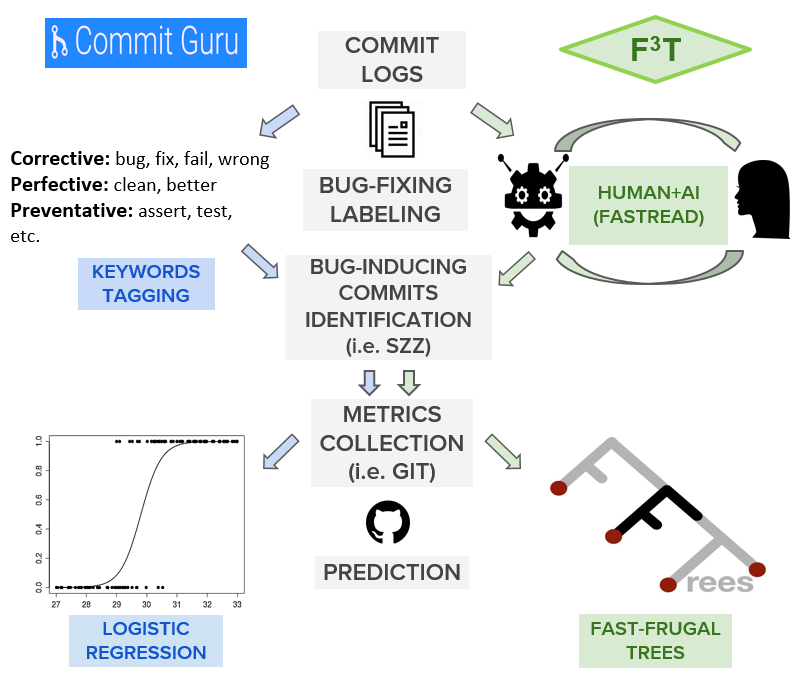
\includegraphics[width=\linewidth]{summary.PNG}
\vspace{-14pt}
\caption{Summarized data mining pipeline of $F^3T$ versus the state-of-the-art system (i.e. Commit.Guru \cite{commitguru}) for risky software commit prediction. Blue left flow represents Commit.Guru system while Green right flow represents our recommended system, $F^3T$.}\label{fig:system}
\vspace{-6mm}
\end{figure} 

\begin{table*}[!t]
\caption{Commit messages from computational
software systems (see~\tbl{data}). Each commit is labeled ``worrying'' by either
a keyword method (from Commit.Guru\cite{commitguru})) or FASTREAD (from our proposed $F^3T$ method). 
Right-hand side comments comes from a manual inspection of each commit.} 
\scriptsize
\begin{center}
\vspace{-5pt}
\hspace{-5pt}\resizebox{1.02\linewidth}{!}{
\begin{tabular}{l|cc|c}
 &  \multicolumn{2}{|c|}{\small{Label=``worrying''?}} & \small{Comment on the}\\

\small{Commit message} & \small{Keyword} & \small{FASTREAD} & \small{Keyword labels}\\ 
\hline
%\texttt{fixed: rmsd\_fit\_trj() failed to write a XTC file} & Y & Y &   \\ 
\texttt{fixes \#143: alignto() now checks the 2 selections describe the same atom} & Y &	 Y &   \\ 
\texttt{Correct bugs due to merge (rhotoxc)}	& Y &	 Y & \small{Correct}\\ 
\texttt{Convert tsmear to tphysel in vtorhotf.F90} &	 N &	 N &  \\ 
\texttt{Universe can load multiple trajectories from positional args} &	 N &	 N &   \\ \hline
\texttt{NetCDFWriter working (closes Issue 109)}	& N&	 Y &  \\ 
\texttt{Correction in magnetization rotation (DFPT+PAW)} &	 N &	 Y &  \\
\texttt{Add missing module dependency} &	 N &	 Y & \small{False-Negative}\\ 
\texttt{findSubgraphIsomorphisms works if you pass it a complete mapping} &	 N &	 Y &  \\ 
%\texttt{Test for issue \#352 now pass} &	 N &	 Y &  \\ 
\hline
\texttt{documentation updates and fixes} &	 Y &	 N &   \\ 
\texttt{Removed unused expected error from Selections} &	 Y &	 N &   \\ 
\texttt{Test for HOLE changed form error to warning when HOLE binary is not there} &	 Y &	 N & \small{False-Positive}  \\ 
\texttt{Added CHANGELOG entry for fix of Issue \#550.} &	 Y &	 N &  \\ 
%\texttt{Make error message clearer in tests for TPR parser} &	 Y &	 N &   \\ 
\hline
\end{tabular}}
\label{tbl:sample}
\end{center} 

 
\end{table*}




% \begin{table*}
% {\scriptsize
% \begin{center}
% \caption{Commit labelled  ``worrying'' by 
% a keyword method (from Commit.Guru\cite{commitguru})) or   $F^3T$. 
% Right-hand side comment comes from a manual inspection.}
% \begin{tabular}{l|cc|c}
%   \rowcolor{gray!30}               & \multicolumn{2}{|c|}{Label=``worrying?''} & Comment on the\\
%  \rowcolor{gray!30} Commit message & Keyword & $F^3T$ &  Keyword labels\\ 
% \hline
% \texttt{fixed: rmsd\_fit\_trj() failed to write a XTC file} & y & y &   \\ 
% \texttt{fixes Issue 143: alignto() now checks that the two selections describe the same atoms} & y &	y &   \\ 
% \texttt{Correct bugs due to merge (rhotoxc)}	& y &	y & Correct\\ 
% \texttt{Convert tsmear to tphysel in vtorhotf.F90} &	n &	n &  \\ 
% \texttt{Universe can load multiple trajectories from positional args} &	n &	n &   \\ \hline
% \texttt{NetCDFWriter working (closes Issue 109)}	& n &	y &  \\ 
% \texttt{Correction in magnetization rotation (DFPT+PAW)} &	n &	y &  \\
% \texttt{Add missing module dependency} &	n &	y & False-Negative\\ 
% \texttt{Correct dfptnl\_pert.F90 for parallel computations} &	n &	y &  \\ 
% \texttt{Test for issue \#352 now pass} &	n &	y &  \\ \hline
% \texttt{documentation updates and fixes} &	y &	n &   \\ 
% \texttt{Removed unused expected error from Selections} &	y &	n &   \\ 
% \texttt{Test for HOLE changed form error to warning when HOLE binaray is not there} &	y &	n & False-Positive  \\ 
% \texttt{Added CHANGELOG entry for fix of Issue \#550.} &	y &	n &  \\ 
% \texttt{Make error message clearer in tests for TPR parser} &	y &	n &   \\ \hline
% \end{tabular}
% \label{tbl:sample}
% \end{center} }
% \end{table*}
%These commit messages include specialized grammars and contents.
% Current practice of developers in software maintenance involved them describing these maintenance in commit messages.


One important aspect of software maintenance is to find the defects within the software in order to allocate relevant resources to fix it and  approximate the trend how the defects occur for bettering future practices of software maintenance \cite{menzies10dp, menzies07dp, ambros10extensive, nagappan05codechurn,elbaum00codechurn, moser08changemetrics, hassan09codechanges}.  Due to the importance of defect prediction, numerous studies this past decade proposed methods to help identify defects. Researchers have analyzed source code (e.g., by code metrics or code smells) \cite{menzies07defect, menzies10dp, ambros10extensive}, or source code comments and commit messages introduced by a developer intentionally describing their work \cite{mockus00changeskeys, hindle08_largecommits, Kim08changes, kamei12_jit}. For e.g., one commit in the ABINIT project is ``\texttt{Fixed bug in DDB interpolation}'' indicates that the corresponding code was ``fixed'' just now to handle DDB interpolation. Therefore, before the patch of this issue got fixed, the previous code has bugs and researchers applied  (1) Sliwerski, Zimmermann, and Zeller algorithm (SZZ)  traced back the commit that introduced the bugs \cite{costa17szz, Kim08changes, Sliwerski05changes}, (2) collect the metrics associated with the bugs \cite{menzies07dp, commitguru, kamei12_jit}, (3) build defect predictors on them \cite{agrawal2018better, di18_fft, Tu18Tuning, ghotra15}. 
Figure \ref{fig:system} shows this pipeline,
bas instantiated by the Commit.Guru tool~\cite{commitguru} (illustrated as the blue flow). 

%The premise of this paper is that, apart from the problem addressed by SZZ, there is {\em another} part of the Figure \ref{fig:system}  that deserves more attention.
Most prior research in software analytics focuses on bug-inducing commits identification, metrics collection, and prediction (the later parts of the pipeline). The problem of automating labeling these commits in Table \ref{tab:words}  is rarely explored, even though this step is the primary task of Figure \ref{fig:system} to get the ``right'' data for consequent tasks. Current practice in software analytics is to categorize these commit messages via the set intersection of the text against a list of keywords (see Table \ref{tab:words}). Vasilescu et al. \cite{Vasilescu15github} remarked that this categorization process is central for researchers to generating defect prediction learning on changes level \cite{commitguru, Kim08changes, catolino17_jitmobile, nayrolles18_clever} regardless of studies showing low accuracy performance even with the help of topic modeling \cite{fu05committopic}. For instance, Table \ref{tbl:sample} shows decisions of 15 commit messages and a lot of them can be incorrectly labeled by the traditional automatic
keyword approach (i.e. looking for presence of the Table \ref{tab:words} terms in the commit message).  It is timely to call for an empirical study for assessing and exploring the labeling process for software analytics, especially risky software commits prediction. Hence, this paper and our recommended system, $F^3T$ (illustrated as the green flow in Figure \ref{fig:system}).

 
 %``risky, not risky''\footnote{Which is Commit.Guru's way of denoting "buggy" or "not buggy".} 
 





%Deciding which commits are bug-fixing can be quite complex. 


 
 
%without exploring and assessing the labeling process which is the first and foremost step in the pipeline to collect the ``right'' data (i.e., bug-fixing commits as the first step in the pipeline). 


%They further remark that while the categorization process is central to tasks such as generating defect predictors, only few papers rigorously explore this categorization process. 
%The current trend of researching approaches include (1) tracing the right commit that introduces the bug (i.e. SZZ) \cite{costa17szz, Kim08changes, Sliwerski05changes} and (2) collecting bugs' metrics and building data miners \cite{yan18_tddetermination, kamei12_jit, nayrolles18_clever, catolino17_jitmobile, yan18_tddetermination, commitguru} 



%Moreover, , it is aligned with Agrawal et al. \cite{agrawal2018better} reported that fixing the weaker regions of the training data in SE defect prediction data can improve the performances on multiple criterias (e.g. AUC and recall drastically).

%This paper address the challenge raised by Vasilescu. We conducted a detailed examination of the process of categorizing comments to find that:

%\bi
%\item Purely automatic methods that just use keywords from Table \ref{tab:words} should be deprecated;
%\item Manual methods where humans reflect more on the commit messages and their categorization are recommended.
%\ei

This work essentially addresses the challenges raised by Vasilescu et al. \cite{Vasilescu15github}. They recommended that the process is explored in an iterative manner where commit categories are studied manually as human engineers adjust the regular expressions containing these keywords.  We conducted a detailed examination of the process of categorizing comments to find that purely automatic method that merely uses syntactic criteria like  {\em words} from Table \ref{tab:words} can perform worse than the {\em combination} of Human+AI. At least in the particular case of studying textual artifacts from software projects, humans have more insight into those artifacts that AI.  More generally, we caution that humans should never be replaced by just AI algorithms. 

\begin{table}
\small
\caption{Words and Categories for Classifying Commits \cite{hindle08_largecommits}}\label{tab:words}
\vspace{-10pt}
 {\footnotesize \begin{tabular}{l|l}
\textbf{Category}  & \textbf{Associated Words}    \\\hline
Corrective & \texttt{bug, fix, wrong, error, fail, problem, patch} \\
Feature Addition & \texttt{new, add, requirement, initial, create} \\
Merge & \texttt{merge} \\
Non Functional & \texttt{doc} \\
Perfective & \texttt{clean, better} \\  
Preventive & \texttt{test, junit, coverage, asset} \\
\end{tabular}}
\vspace{-8mm}
\end{table}



That said,  adding humans into an analytic process is time-consuming. In the sample of commit messages explored by this study, commit messages are two to four lines long, and these can be read and critiques by humans at a rate of no more than ten per minute. This means that while automatic tools can read a billion commit messages in a minute, humans struggle to analyze ten. Hence, before we can advocate partnerships of human and artificial intelligence for software analytic, we must somehow manage and minimize the work required by the human partner.

Accordingly, this paper explores {\em active learning} methods to implement the human+AI partnership. The key idea behind active learning is that a machine learning algorithm can train faster (i.e., using less data) if it is allowed to choose the data from which it learns~\cite{settles2012active}. The experience in other domains is that such active learners can significantly reduce the amount of effort required to achieve high recall~\cite{Cormack2017Navigating, Cormack2016Engineering, cormack2016scalability, Cormack2015Autonomy, Cormack2014Evaluation, Wallace2010Semi, wallace2010active, wallace2011should, wallace2012class, nguyen2015combining, Yu2018Recall}. Our approach initially uses uncertainty sampling to fast build a reliable model, then switches to certainty sampling to greedily find buggy commits files. This strategy significantly reduces the effort required to find some desired level of high recall of buggy commits.

To test this approach, we categorized $45,000+$ commits from nine different computational softwares using (a)~the standard keyword methods and (b)~the active learning method described previously. 

Data acquisition comes prediction.  State-of-the-art data mining methods for software analytics include Synthetic Minority Oversampling Techniques (SMOTE) to handle class imbalance \cite{agrawal2018better, kamei12_jit} in combination with standard miners (Random Forest (RF), Logistic Regression (LR), and Support Vector Machine (SVM)). However, Chen et al. \cite{di18_fft} recommended Fast-Frugal Trees as the prediction model where it demonstrated that the model have dominated other standard methods for defect prediction and close issues prediction. Therefore, our recommended system to explore and improve the state-of-the-art risky software prediction of $F^3T$ as the combination of FASTREAD labeling method and FFTs predicting model will be validated with the comparisons against other standard data mining methods and answering the following research questions:

\textbf{RQ1: { How close are FASTREAD and Keyword Labeling to Human Labeling?}}
 
Software maintenance is a continuing process, and software developers have the domain expertise in understanding the commit logs. 25,000+ commits are crossed labeled by SE Ph.D. students from 4 projects. With the initial assumption that software maintenance requires the expert's understanding, these human-labeled commit logs data from those four initial sampled repositories serves as the ground truth to compare the effectiveness of automatic Keywords versus FASTREAD tagging. FASTREAD statistically significant won across four cases with our three evaluation metrics of precision, recall, and false-alarms (up to 38\% precision, 31\% recall and 111\% false-alarm).
 
 %Four popular repositories that satisfy our sanity checks were picked at random, and their commit logs were sampled to be labeled for bug-fixing commits by a human. 

\begin{RQ}{}
\vspace{-10pt}

FASTREAD as the method for bug-fixing commits augmentation is better than current automatic keyword tagging.
\end{RQ}
 
 
 \textbf{RQ2: { How are risky software commit prediction based on FASTREAD labeled data perform against state-of-the-art method (Keyword) labeled data?}}
  
%From the bug-fixing commits, we can track back to find bug-inducing commits that introducing defects to the software. Each of these commits will be analyzed, and recommended metrics are extracted to describe how risky each commit is. 

The right green flow in Figure \ref{fig:system} demonstrated our approach to improve the correctness of finding the bug-fixing commits. When the right bug-inducing commits are linked and analyzed to extract relevant values of metrics, a more robust model to predict future risky software commits is built. FFTs is validated as our chosen data miner when FFTs dominated the three standard methods (SMOTE+RF, SMOTE+LR, and SMOTE+SVM) in our experiment described in section 4 (RQ2). By winning 7 (78\%) for G-value and 6 (67\%) for $P_{opt}$ out of 9 projects, FFTs model built on FASTREAD labeled data outperform FFTs model built on Keyword labeled data. 
 

\begin{RQ}{}
\vspace{-10pt}
FASTREAD labeled data are more fit and higher quality for risky software commit prediction. Automatic Keywords labeling method for defective software commit is deprecated for future defect prediction work.  
\end{RQ}
  

\textbf{RQ3: {How state-of-the-art risky software commit identification and prediction system, Commit.Guru, comparing to our recommended $F^3T$ system in predicting risky software commit?}}
 
%Data quality also comes from the proportion of the labels within the dataset. Agrawal et al. \cite{agrawal2018better} has found that imbalance class problem is apparent within defect prediction research. Although our study is not defect prediction, it does inherit a lot of defect prediction problem's nature where most of the commits are not bug-inducing commits. Risky software commit prediction also exhibit an imbalance class problem. Outside of data quality, data miner should be chosen carefully to leverage the nature of the problem and the dataset itself. 

Current state-of-the-art risky software commit identification and prediction system is Commit.Guru (Keyword + Logistic Regression) that illustrated in the left blue flow in Figure \ref{fig:system}. However, FASTREAD is proven to improve the dependent features quality, or the correctness of risky software commit identification, the target for prediction task (from RQ1 and RQ2) while FFT has proven to be a robust data miner for software analytics task. Our proposed system of $F^3T$ (FASTREAD+FFTs) dominated on G-values with statistically significants win on all 9 projects and improvement  of the absolute delta up to 48\%. For $P_{opt}$,  $F^3T$ won 7 out of 9 projects with the absolute delta up to 26\%. 

  
\begin{RQ}{}
\vspace{-10pt}
$F^3T$ outperformed state-of-the-art risky software commit identification and prediction system, Commit.Guru. $F^3T$ is recommended as a new baseline for future research work.
\end{RQ}

%  \textbf{RQ4: { How the FFT model comparing to state-of-the-art methods in predicting risky software commit?}}
 
%  Modern state-of-the-art methods do include more than just Logistic Regression such as Random Forest (RF) and Support Vector Machine (SVM) for more complex problems in combination with Synthetic Minority Oversampling Technique (SMOTE) to handle class imbalance problem. It is essential to validate our data miner of choice FFT by comparing it against state-of-the-art data miners. With seven wins, one loss, and one tie, FFT model outperformed state of the art data miner in risky software commit prediction.  

 
% \begin{RQ}{}
% \vspace{-10pt}
% FFT model outperformed state-of-the-art risky software commit prediction and is recommended as a new baseline for future work in risky software commit prediction.
% \end{RQ}

\noindent
In summary, the main contributions of this paper are:
\bi
% \\item 
% \item Fastread labeling offer higher quality data for predicting risky software commit than state-of-the-art labeling method, Commit.Guru's automatic keyword labeling.  
% \item FFT as a recommended data mining model offer better improvement of performance scores than state-of-the-art methods, Commit.Guru's Logistic Regression. 
\item A first novel inter-disciplinary contribution of human+AI partnership and psychological science in software quality assurance. 
\item A demonstration of Human+AI partnership for software analytics outperforming approaches that are solely abusing AI. 
\item An assessment of active learning for data ingestion quality problem by reproducing prior approach and comparing it with our recommended system.  
\item A reproduction package containing all the data and algorithms of this paper, see \url{https://github.com/anonymous-for-review}.
\ei



The rest of this paper is structured as follows. Background work is discussed  in section 2. 3 describes our empirical methodology and experimental design.  This is followed by the details of the experiment results while answers the research questions. Threats are analyzed in 5. future work is provided in 6. 



\section{Background}

\subsection{Defect Commit Logs Labeling}

Through software development and maintenance, developers are supported to describe their work that were pushed through commit messages. One popular practice of identifying or reasoning the rate of bugs is searching for defect-related keywords through these messages \cite{mockus00changeskeys, hindle08_largecommits}. It has been adopted in empirical SE research extensively without rigorous critique (e.g., \cite{nayrolles18_clever, catolino17_jitmobile, kamei12_jit, Kim08changes}). Does this set of keywords can be generalized to the diverse community of SE research? 

According to Fu et al., even with the full automation through topic modeling, the accuracy performance was low \cite{fu05committopic}. For instance, this study specifically focuses on softwares from computational science (which is elaborated more in section 3.1) and Keyword automatic labeling method that have performed well in SE researches \cite{commitguru, nayrolles18_clever, Kim08changes, kamei12_jit} made fatal mistakes as recorded in Table \ref{tbl:sample}. There are indeed agreements between state-of-the-art keywords labeling and human+AI (i.e. FASTREAD column) that can be observed in the first 5 entries of Table \ref{tbl:sample}. However, for ``\texttt{Make error message clearer in tests for TPR parser}'' would be marked as bug-fixing commit and the commit introduces the code that being changed will be marked as buggy and the data miner will learn not relevant metrics to identify risky commit, which is a false-positive example. Moreover, such commits as ``\texttt{NetCDFWriter working (closes Issue 109)}'' was not marked as bug-fixing commit by the state-of-the-art keywords but it was indeed a bug-fixing one so the data associated with risky commit was not collected and learned for the data miner, which is a false-negative example. These mistakes conjectured that the standard Keyword automatic labeling in SE failed to fully capture the semantics of these commits. Instead of going for full-automation for too low of relevancy or full-human for too expensive of labor work, the data ingestion and other studies \cite{costa17szz, Kim08changes, nayrolles18_clever, catolino17_jitmobile, kamei12_jit, kamei12_jit} that utilize it can improve by combining both manual and automating approaches for identifying bug-fixing commits, human-in-the-loop AI or human+AI partnership. Formally, the problem explored in this paper can be expressed using the nomenclature of Table 2:
\bi
\item Starting with $L = \emptyset$ commits;
\item Prioritize which commits to be reviewed in order to 
\begin{enumerate}
    \item maximize $|L_{R}|$ (the number of relevant or bug-fixing commits discovered)
    \item while minimizing $|L|$ (the number of commits reviewed).
\end{enumerate}
\ei


\begin{table}[!t]
\footnotesize
\caption{Problem description}
\vspace{-10pt}
\label{tab: problem}
\begin{tabular}{ll}
\rowcolor{gray!10} 
$E$: & the set of all candidate commits (returned from search).\\\rowcolor{gray!10} 
$R\subset E$: & the set of ground truth bug-fixing commits. \\\rowcolor{gray!10} 
$I=E\setminus R$: & the set of ground truth not bug-fixing commits.\\\rowcolor{gray!10} 
$L\subset E$: & the set of labeled/reviewed commits, \\\rowcolor{gray!10}  & each review reveals whether a commit $x\in R$.\\\rowcolor{gray!10} 
$\neg L=E\setminus L$: & the set of unlabeled/unreviewed commits.\\\rowcolor{gray!10} 
$L_R=L\cap R$: & the identified bug-fixing (included) commits.\\\rowcolor{gray!10} 
$L_I=L\cap I$: & the identified not bug-fixing (excluded) commits.
\end{tabular}
\vspace{-5mm}
\end{table}


In order to achieve the combination, {\em active learning} is adapted. It can train faster (i.e. using less  data) if it is allowed to choose the data from which it learns~\cite{settles2012active}. The experience in other domains in literature reviewing task (e.g. legal reasoning, evidence-based medicine, and software engineering) is that such active learners can significantly reduce the amount of effort required to achieve high recall~\cite{Cormack2017Navigating, Cormack2016Engineering, cormack2016scalability, Cormack2015Autonomy, Cormack2014Evaluation, Wallace2010Semi, wallace2010active, wallace2011should, wallace2012class, nguyen2015combining, Yu2018Recall}. Systematic literature review specifically in SE is a manual process till recent development of automatic tool support FASTREAD that utilize active learning. 

 

Firstly, to understand how FASTREAD was designed with active learning for smart and efficient bug-fixing commits labeling, consider the FASTREAD algorithm \cite{Yu2018} starting with the decision plane between the bug-fixing commits and other commits in \fig{svm}. Suppose we want to find more buggy commits and we had access to, say, a support vector machine (SVM) model built from some examples seen to date. 
One tactic for quickly finding those buggy commits would be to ask humans to review and assess a few dozens \begin{wrapfigure}{r}{1.3in}
\vspace{-10pt}
\hspace{-12pt}
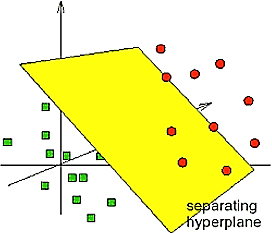
\includegraphics[width=1.4in]{svm.png}
\vspace{-5pt} \hspace{-25pt} \caption{ Separating risky (red) from  non-risky (green) files.}\label{fig:svm}
\vspace{-15pt}
\end{wrapfigure}  of commits that fall into the red region of this figure, as far as possible from the green ones (i.e. {\em certainty sampling}). Another tactic would be to verify the position of the boundary, inspect unclassified files that are closest to the boundary (i.e. {\em uncertainty sampling}). Our approach initially uses uncertainty sampling to fast build a reliable model, then switches to certainty sampling to greedily find bug-fixing commits. Holistically,  the machine learner (i.e. SVM) use this feedback from human to learn their models incrementally. These models are then used to sort the stream of commit messages such that humans read the most informative ones first. This strategy significantly reduces the effort required to find some desired level of high recall of buggy commits.

FASTREAD was designed and evaluated after testing and comparing against 32 different active learners generated from three prior state of the art methods from the medical and legal literature - Wallace et al. and Cormack et al. \cite{wallace2010active, Cormack2015Autonomy}. FASTREAD dramatically reduces manual reading methods (linear review) by an order of magnitude fewer papers are required to be reviewed to find 95\% of the relevant ones. When compared to current state of the art automatic methods - Wallace and Cormack \cite{wallace2010active, Cormack2015Autonomy}, FASTREAD reviews up to 50\% fewer papers while finding the same number of relevant papers. While FASTREAD is proven to be effective in reducing efforts for reviewing literature, defect prediction can benefit from FASTREAD to build a personalized topic model for the specific project to identify the bug-fixing commits.  




% \begin{algorithm}[!t]
% \footnotesize
% \SetKwInOut{Input}{Input}
% \SetKwInOut{Output}{Output}
% \SetKwInOut{Parameter}{Parameter}
% \SetKwRepeat{Do}{do}{while}
% \Input{$E$, set of all candidate papers\\$R$, set of ground truth relevant papers}
% \Output{$L_R$, set of included papers}
% \BlankLine

% $L\leftarrow \emptyset$\; $L_R\leftarrow \emptyset$\; $\neg L\leftarrow E$\; 

% \BlankLine
% \tcp{Keep reviewing until stopping rule satisfied}
% \While{$|L_R| < 0.95|R|$}{
%     \tcp{Start training or not}
%     \eIf{$|L_R| \geq 1$}{
%         $CL\leftarrow Train(L)$\;
%         \tcp{Query next}
%         $x\leftarrow Query(CL,\neg L,L_R)$\;
%     }{
%         \tcp{Random Sampling}
%         $x\leftarrow Random(\neg L)$\;
%     }
%     \tcp{Simulate review}
%     $L_R,L\leftarrow Include(x,R,L_R,L)$\;
%     $\neg L\leftarrow E \setminus L$\;
% }
% \Return{$L_R$}\;
% \BlankLine
% \Fn{Train($L$)}{
%     \tcp{Train linear SVM with Weighting}
%     $CL\leftarrow SVM(L,kernel=linear,class\_weight=balanced)$\;
%     \If{$L_R\ge 30$}{
%         \tcp{Aggressive undersampling}
%         $L_I\leftarrow L\setminus L_R$\;
%         $tmp\leftarrow L_I[argsort(CL.decision\_function(L_I))[:|L_R|]]$\;
%         $CL\leftarrow SVM(L_R \cup tmp,kernel=linear)$\;
%     }
%     \Return{$CL$}\;
% }
% \BlankLine
% \Fn{Query($CL,\neg L,L_R$)}{
%     \eIf{$L_R< 10$}{
%         \tcp{Uncertainty Sampling}
%         $x\leftarrow argsort(abs(CL.decision\_function(\neg L)))[0]$\;
%     }{
%         \tcp{Certainty Sampling}
%         $x\leftarrow argsort(CL.decision\_function(\neg L))[-1]$\;
%     }
%     \Return{$x$}\;
% }
% \BlankLine
% \Fn{Include($x,R,L_R,L$)}{
%     $L\leftarrow L \cup x$\;
%     \If{$x\in R$}{
%         $L_R\leftarrow L_R \cup x$\;
%     }
%     \Return{$L_R$, L}\;
% }
% \caption{ FASTREAD~\cite{Yu2018}}\label{alg:alg1}
% \end{algorithm}

\begin{table*}[!t]
\small
\centering
\caption{14 independent studied features for software maintenance changes \cite{kamei12_jit}.}
\vspace{-10pt}
\label{tbl:metrics}
\resizebox{\linewidth}{!}{
\begin{tabular}{l|l|l|p{12cm}|}
\hline
\rowcolor{gray!60}Dimension & Name & Definition & Rationale \\\hline
\multirow{5}{*}{Diffusion} & NS & Number of modified subsystems & Changes modifying many subsystems are more likely to be defect-prone \\\cline{2-4}
& ND & Number of modified directories & Changes touching more directories
are more likely to introduce defect. \\\cline{2-4}
& NF & Number of modified Files & Changes touching more files
are more likely to introduce defect. \\\cline{2-4}
& Entropy & Number of modified subsystems & Changes with high entropy are more
likely to introduce technical debt, since a developer will
have to recall and track more scattered changes across
each file. \\\hline
\multirow{3}{*}{Size} & LA & Lines of code added & \multirow{2}{*}{Changes touching more lines of code are more likely to introduce defects.} \\\cline{2-3}
& LD & Lines of code deleted & \\\cline{2-4}
& LT & Lines of code in a file before the changes & The larger the file/module, the more likely that the change would be defective. \\\hline
\multirow{2}{*}{Purpose}  & FIX & Whether the change is bug-fixing? & Changes that fixing the defect are more likely to introduce more defects than changes for new functionality implementation. \\\hline
\multirow{5}{*}{History} & NDEV & Number of developers that changed the modified files & Changed files touched by more developers before are more likely to introduce defects, since different developers have different design thoughts and code styles. \\\cline{2-4}
& AGE & The average time interval between the last and the current change & More recent changes (lower age) contribute more defects than older changes (longer age). \\\cline{2-4} 
& NUC & Number of unique changes to the modified files before & Larger NUC changes are more likely to
introduce defects since a developer will have to recall and track many previous changes. \\\hline
\multirow{5}{*}{Experience} & EXP & Developer experience & The experience of developers has an impact on introducing TD \\\cline{2-4}
& REXP & Recent developer experience & The experience of developers that has often modified the files are less likely to introduce defects (more familiar with the system).  \\\cline{2-4}
& SEXP & Developer experience on a subsystem & Modifications that are made by developer that are familiar with the subsystems are less likely to introduce defects.  \\\cline{1-4}

\end{tabular}}
\vspace{-7pt}
\end{table*}

\subsection{Defect Prediction Past and Now}

In 2007, the market for software tools and services has been growing to \$300 million, with 50 to 83 percent increases in static analysis and black-box testing sectors. More robust and secure software is necessary as this trend continues. Software faults and
failures were estimated by the US National Institute of
Standards and Technology (NIST) that  \$60 billion a year in the US \cite{softwareecon}. 

Therefore, significant SE research has focused on software analytics and the prediction of software quality. Data about the development process (e.g., code and/or repository data) is trained to provide software analytics. In fact, in the past decade more than a hundred paper were published on software defect prediction alone \cite{sedp100}. Consequently, detecting the existence of defects in software projects an evergreen research field with 5 popular research paths:
\begin{enumerate}
    \item Predict the location of defects so that appropriate resources may be allocated (e.g., Bird et al \cite{bird09reliabity})
    \item Understand the factors that lead to greater likelihood of defects such as defect prone software components using code metrics (e.g., ratio comment to code, cyclomatic complexity) \cite{menzies10dp, menzies07dp, ambros10extensive} or process metrics (e.g., number of changes, recent activity) \cite{nagappan05codechurn,elbaum00codechurn, moser08changemetrics, hassan09codechanges}.
    \item Enhance discriminatory the power of the traditional approaches in finding the defects in software systems \cite{ghotra15}. This has led to development of hyperparameter optimization and better data harvesting tools \cite{agrawal2018wrong, agrawal2018better, Fu17easy, Fu16Grid, Fu2016TuningFS}. 
    \item Use defect prediction to proactively fix these defects, such as the automated program repair research area \cite{kamei16_lit, legoues12_aprlit, arcuri2011practical}. 
    \item Study defect prediction not only just release-level \cite{di18_fft, agrawal2018better} but also change-level or just-in-time \cite{yan18_tddetermination, kamei12_jit, nayrolles18_clever, commitguru} both for research and also industry.  
\end{enumerate}



\subsection{Risky Software Commit Prediction}

Previous studies have focused on the prediction of risky software changes for short-term quality assurance. Mockus and Weiss predicted the risk of a software change at coarse-grained granularity in an industrial project with features such as \# of subsystems touched,\# of files modified, \# of modification requests. Through studying defect-introducing changes in the Mozilla and Eclipse, Sliwerski \cite{Sliwerski05changes} found that large transaction of code would include defect and changes done on specific time have a higher change of introducing defects, especially Friday. Eyolfson et al. \cite{Eyolfson11bugginess} noted that software changes performed late night (between midnight and 4 AM) are more buggy than changes committed morning (7 AM and noon) and that developers who commit regularly produce less buggy changes.  A study
that characterizing incorrect defect fixes in Linux, OpenSolaris, FreeBSD, and a commercial operating system by Yin et al. \cite{Yin11fixes} found that 14.8\%-24.2\%  of fixes are incorrect and affect end users, that concurrency defects are the most difficult to fix, and that developers responsible for incorrect fixes usually do not have enough knowledge about the code being changed.

Inspired by their work, Kamei et al. did a large scale study of the Just-in-time (JIT) software change on a set of 6 open source projects and 5 commercial projects through the 14 metrics categorized into 5 dimensions of diffusion, size, purpose, history, and experience  \cite{kamei12_jit}. To the most recent work, Kim et al. \cite{Kim08changes} sampled a balanced subset of changes and use source code change logs in several open source projects and obtained 78 percent
accuracy and a 60 percent recall. However, Kamei's work use the combination of change logs and the change metrics, reported in Table \ref{tbl:metrics}, predicting defect-inducing chnages with 68\% accuracy and 64\% recall with lower fraction bug inducing changes. 
Barnett et al. extended Commit.Guru to include commit volume and Naive-Bayes (NB) score on how risky a commit content is on 342 MSR coding data challenge repositories to incorporate the relationship between commit message detail and defect pronerective, adaptive, or perfective issues \cite{barnett13_mcontent}.  

Rosen et al. developed by a tool called Commit.Guru ~\cite{commitguru} to identify ``risky'' commits have made change-level defect prediction research path more accessible (the system is described in the blue flow of Figure \ref{fig:system}). They categorized actions undertaken by commits based on a list of verbs present in the messages into five categories (a) corrective action, (b) feature addition, (c) merge, (d) documentation, and (e) perfective and preventative measures. The LR model is used for classification task by building it on top of  stemmed from prior work  that are shown in Figure \ref{tbl:metrics}. 
 
Previous work have sparked change-level bug level in different domains in software analytics. In 2017, Catolino \cite{catolino17_jitmobile} evaluated metrics proposed by Kamei et al. \cite{kamei12_jit} for JIT bug level for mobile applications domain with 5 open-source mobile applications where they found only a subset of 5 metrics were considered meaningful including: \# modified subsystems, \# added LOC, \# LOC before the commit, \# developers working on the committed files, experience of the developer. Through LR for modeling, they achieved 70\% accuracy but 17\%-38\% for recall. In 2018, Nayrolles et al. \cite{nayrolles18_clever} extends Commit.Guru to build the CLEVER (Combining Levels of Bug Prevention and Resolution techniques) tool experimenting on 12 Ubisoft software projects to help repair the program more proactively. Instead of LR, they classify the commit risky or no-risky based on Random Forest algorithm. If the commit is risky, they then comparing commit code blocks with NICAD code clone detector \cite{cordy11_NiCad} of software clones with similar defect-introducing commit and proposed the associated bug-fixing commit as the potential fix to the developer. Yan et al. \cite{yan18_tddetermination} studied 7 projects at change-level for technical-debt (TD) introducing changes of Hadoop, Ant, Camel, Jmeter, Log4j, Tomcat, and Gerrit from 0.75\% to 4.22\% targeted TD-introducing changes. They extended 13 features studied by Kamei et. al \cite{kamei12_jit} to 25 changes features categorized into Diffusion, History, and Message with $FA, FM, FD, FR, FC$, $LCC, MCC, HCC,$ and $CCC$ calculated by ChangeDistiller \cite{fluri07_changedistiller}. They applied NB and RF model to train and determine TD-introducing changes. Diffusion is the most discriminating features set to learn TD-introducing changes with AUC score of 82\% and cost-effectiveness of 80\%.


From all of the above work, we noticed: 
\begin{enumerate}
    \item None questioning the full automation nature of dependent feature acquisition (bug-fixing commits identification through keyword tagging), i.e. buggy or non-buggy software changes for risky commit prediction model. Barnett et al. found that 43\% and 80\% of the JIT models of the studied systems are significantly improved by incorporating the relationship between commit message detail and defect proneness \cite{barnett13_mcontent}. Yet, independent metric FIX and bug-fixing status of a commit (for future tracing the risky software commits as the targets) are done by automatically searching for the existence of the defect-related keywords in the commit messages even when discouraged by low performance with support of topic modeling. Our work shall augment the bug-fixing status of the commits by FASTREAD method to improve the quality of dependent features of the risky software change prediction data. 
    \item Only the large scale study done by Kamei et al. \cite{kamei12_jit} mentioned how to deal with imbalance class problem nature of defective change-level prediction by resampling approach to randomly delete instances from the majority category. Our experiment will incorporate state-of-the-art imbalance class handling technique, Synthetic Minority Oversampling Technique (SMOTE). 
    \item They only applying LR, NB, and FR as their data mining method. Our work also compare with SVM while introducing state-of-the-art data mining model of Fast-Frugal Trees for risky software commit prediction.    
\end{enumerate}

\begin{figure}[!b]

 {\normalsize
\begin{minipage}{\linewidth}
\vspace{-5mm}
\begin{tabular}{p{\linewidth}}
  \texttt{\qquad  if  \qquad \ \ \ LA $<$  10   \qquad \qquad  \ then false \qquad \#0} \\
  \texttt{\qquad  else if \ \ Entropy $\geq$  0.65    \ \      then true \qquad \  \#1} \\
   \texttt{\qquad else if \ \ NS $>$  3   \qquad \qquad \ \   then true \qquad \  \#1} \\
   \texttt{\qquad else if \ \ FIX $==$ 1    \qquad \qquad  then true \qquad \  \#1} \\
   \texttt{\qquad else \qquad \qquad \qquad \qquad \ \ \ \ \ \ \ false \ \  \ \ \ \ \ \  \#0} 
\end{tabular}
\end{minipage}
}
\vspace{-5mm}
\caption{Example of an FFT}
\label{fig:fft1}
\end{figure}

\subsection{Fast-Frugal Trees Model in Software Analytics}

Psychological scientists have developed FFTs (Fast and Frugal Trees) as one way to generate comprehensible models consisting of separate tiny rules~\cite{phillips2017fftrees,di18_fft,martignon2008categorization,agrawal18_fft,agrawal2019dodge}. An FFT is a decision tree made for binary classification problem with exactly two branches extending from each node, where either one or both branches is an exit branch leading to a leaf~\cite{martignon2008categorization}. 
 A similar implementation of FFT as offered by Fu and Chen et al.~\cite{fu2018building,di18_fft}. 
An FFT of depth $d$ has a choice of two ``exit policies'' at each level: the existing branch can select for the negation of the target, i.e., not risky, (denoted ``0'') or the target (denoted ``1''), i.e., risky.
The right-hand-side tree in Figure~\ref{fig:fft1} is \texttt{01110} since:
\bi
\item
The first level found a rule that exits to the negation of the target: hence, ``0''.
\item
While the next tree levels exit first to target; hence, ``111''.
\item
And the final line of the model exits
to the opposite of the penultimate line; hence, the final ``0''.
\ei



Following the advice of~\cite{fu2018building,di18_fft,phillips2017fftrees}, for all the experiments of this paper, we use a depth    $d=4$. 
For trees of depth $d=4$, there are $2^4=16$ possible trees which can be denoted as 00001, 00010, 00101, ... , 11110. During FFT training, all $2^d$ trees are generated, then we select the best one (using the training data).
 This single best tree is then applied to the test data.
 Note that FFTs of such small
depths are very succinct
(e.g. Figures~\ref{fig:fft1}). Such FFTs generate rules which leads to decision of finding a report as risky or not risky (defective and non-defective) for the datasets under this study. Chen et al. reported that in comparisons to other standard models in software analytics (SVM, RF, LR, and NB), FFTs performed better in term of $P_{opt}$ and distance to the ``heaven'' point of 100\% recall and no false alarms in at least defect prediction and issue close time prediction  \cite{di18_fft}. Therefore, it is adopted and validated in our study in RQ2 for risky software commit prediction. 

\begin{table}
\small
\begin{center}
\caption{Dataset statistics. Data was mined and curated from each own open project's github repository.}
\vspace{-10pt}

\label{tbl:dataset}
\begin{tabular}{c@{~}|r@{~}|r@{~}|r@{~}|r@{~}}
\begin{tabular}[c]{@{}c@{}} \end{tabular} & \begin{tabular}[c]{@{}c@{}} \textbf{No. of}\end{tabular} & \textbf{No. of} & \textbf{Defective}  \\
 \textbf{Dataset} & \textbf{Commits} & \textbf{Releases} &  \textbf{Commit \%} & \textbf{Source}\\ \hline
HOOMD & 3904 & 8  & 16 & \cite{hoomd} \\ 
LIBMESH & 7801 & 10 & 16 & \cite{libMesh} \\
ABINIT & 3911 & 9 & 18 & \cite{Abinit} \\  
LAMMPS & 5587 & 7 & 18 & \cite{lammps-sandia} \\ 
PCMSOLVER & 1655 & 2  & 23 & \cite{pcmsolver}  \\ 
AMBER & 4243 & 4  & 23 & \cite{Amber-MD} \\ 
RMG-PY & 4472 & 7 & 27 & \cite{ReactionMechanismGenerator}  \\ 
MDANALYSIS & 2733 & 8  & 37 & \cite{mdanalysis}  \\  
XENON & 1804 & 7  & 46 & \cite{xenon} \\ 


\end{tabular}
\end{center}
\vspace{-10pt}
\end{table}

\section{Experimentation}

\subsection{Dataset}

This study investigates the software development of Computational Science softwares.  678 projects were collected from different sources including internal labor source of NSF $SI^2$ survey, individuals \footnote{Wolfgang Bangerth}, and organizations \footnote{The Molecular Sciences Software Institute (MOLSSI), and Science Gateways Community institute (SGCI)}. These standard sanity checks (of Table~\ref{tbl:sanity}) were taken and adapted from studies \cite{bird09promise,agrawal2018we, eirini15promise, munaiah17curating} to narrowing down the projects that contain sufficient software development information. From the initial pool of 678 projects, 55 targeted open-source projects are decided. This paper collected data from a sample of nine projects within that pool having $36,000$ change commits chosen to cover a range of languages (Java, Python, C/C++, and Fortran), summarized in Table \ref{tbl:dataset}.

% \bi
% \item PCMSolver (PCMSOLVER): An API for the Polarizable Continuum Model \cite{pcmsolver}.
% \item Xenon: A middleware abstraction library that provides a simple programming interface to various compute and storage resources \cite{xenon}.

% \item MDAnalysis (MDANALYSIS): a Python library to analyze molecular dynamics trajectories generated by a wide range of popular simulation packages \cite{mdanalysis}.
% \item HOOMD-blue (HOOMD): a general purpose particle simulation toolkit. It performs hard particle Monte Carlo simulations of a variety of shape classes, and molecular dynamics simulations of particles with a range of pair, bond, angle, and other potentials \cite{hoomd}.  
% \item ABINIT (ABINIT): an atomic-scale simulation software suite \cite{Abinit}.
% \item Amber (AMBER): Fast, parallelized molecular dynamics trajectory data analysis \cite{Amber-MD}.

% \item RMG-py (RMG-PY): Python version of Reaction Mechanism Generator, a tool for automatically generating chemical reaction mechanisms for modeling reaction systems including pyrolysis, combustion, atmospheric science, and more \cite{ReactionMechanismGenerator}.
% \item LAMMPS (LAMMPS): Large-scale Atomic/Molecular Massively Parallel Simulator, a classical molecular dynamics simulation code \cite{lammps-sandia}.
% \item libMesh (LIBMESH): a framework for the numerical simulation of partial differential equations using arbitrary unstructured discretizations on serial and parallel platforms. A major goal of the library is to provide support for adaptive mesh refinement (AMR) computations in parallel while allowing a research scientist to focus on the physics they are modeling \cite{libMesh}.
% \ei




\begin{table}
\small
\caption{Sanity checks for pruning very small ``hobby'' Github projects.}\label{tbl:sanity}
\vspace{-10pt}
 \begin{tabular}{r|l}
Check   & Condition    \\\hline
Personal purpose (\# Developers) & $>$ 7 \\
Collaboration (Pull requests)  & $>$ 0 \\
Issues & $>$ 10 \\
Releases &  $>$ 1 \\
Commits & $>$ 20 \\
Duration  & $>$ 1 year 
\end{tabular}
\vspace{-17pt}
\end{table}




\subsection{Experimental Rig}

\noindent \textbf{Step 1: Bug-fixing commits augmentation.} For the initial four main projects (ABINIT, libMesh, MDANALYSIS, and LAMMPS), the commit logs are cross-labeled by two graduate students in SE research. Total of 9 projects are augmented by both automatic Keyword tagging method and FASTREAD method. 

\noindent \textbf{Step 2: Bug-inducing change identification.} To link bug-fixing commits and their bug-inducing commits (e.g. crash, bug, issues), the well-known SZZ algorithm that is designed by Sliwerski and improved by Kim et al. is employed \cite{Sliwerski05changes, Kim08changes}.  

\noindent \textbf{Step 3: Metrics Collection.} The recommended 14 metrics to study defect-prone commits by Kamei et al. \cite{kamei12_jit} from Table \ref{tbl:metrics} for each project are recorded by depriving from the source code control system (e.g., Git).  

\noindent \textbf{Step 4: Data Preprocessing.} Current software analytics work include data transformation and prediction. Before experimenting with standard data miners, the data will be ``SMOTEd'' to handle class-imbalance, which was not considered in Commit.Guru. 

\noindent \textbf{Step 5: Data Mining.} We adopted the incremental learning approach for this study where release $i$ of project $j$ is trained and test on release $i+1$. 
For the initial four projects (ABINIT, LIBMESH, LAMMPS, and MDANALYSIS), $j_i[keyword]$ and $j_i[FASTREAD]$ will be trained and test on $j_{i+1}[human]$. From that result, we are confident to scale up without human labels as ground-truth bug-fixing labels. 
Therefore, for the rest five projects, $j_i[keyword]$ and $j_i[FASTREAD]$ \hspace{0.05cm} will be trained to test on \hspace{0.05cm} $j_{i+1}[keyword]$ \hspace{0.05cm} and $j_{i+1}[FASTREAD]$ respectively. 
For this study, we comparing Fast-Frugal Trees against Support Vector Machine, Random Forest, and Logistic Regression (state-of-the-art data miner). The process is repeated 20 times to mitigate biases.  


\subsection{Systematic Commit Logs Labeling}

FASTREAD algorithm \cite{Yu2018} augmented bug-fixing commits by:
\begin{enumerate}
    \item Input thousands of commits per project.
    \item Initial random reasoning phase: humans to skim through the commits messages manually until they have found $|L_R| \geq 1$ bug-fixing commit (along with $|L_I|$ non bug-fixing ones). Dozens of both categories of commits should be found before next step.
    \item Reflective reasoning phase (Line 6-7 \cite{Yu2018})
    \bi
    \item The Support Vector Machine (SVM) model is trained on the $L$ examples. When $|L_R \leq 30|$, aggressive undersampling  are employed to reject all the non bug-fixing commits. 
    \item Uncertainty sampling of commits with highest uncertainty of category when $|L_R \leq 30|$ (line 25) and certainty sampling of commits with highest probability to be bug-fixing when $|L_R \geq 30|$ (line 27).   
    \item Iterate the reflective reasoning phase until more than 95\% of the bug-fixing commits have been found ($|L_R| \geq 0.95|R|$).
    \ei
\end{enumerate}



\subsection{Evaluation Goal}

Ideally, a perfect learner would be able to achieve where all the predicted risky software changes are actually labeled risky are actually positive with no non-risky changes being labeled as risky. Formally, as high recall as possible (up to 100\%) while as low of  false-alarms as possible (down to 0\%). 

\vspace{-5pt}
\begin{equation}
 \mathit{Recall} = \frac{\mathit{TruePositives}}{\mathit{TruePositives} + \mathit{FalseNegatives}}
 \end{equation}
 \vspace{-10pt}
 
\begin{equation}
 \mathit{FalseAlarm Rate(FAR)} = \frac{\mathit{FalsePositive}}{\mathit{TruePositive} + \mathit{TrueNegative}}
 \end{equation}

In order to combine Recall and False-Alarm Rate, we use the the ``G-Score''. Several authors \cite{shatnawi10g1, comments07} have previously shown
that such a measure is justifiably better than other measures
when the test samples have imbalanced distribution in terms
of classes.  G-Score can by computed by measuring the mean
(geometric/harmonic) between the Probability of True Positives
(Recall) and Probability of true negatives (1-FAR). Depending on the variance in Recall/FAR values, it is known that in cases where samples tend to take extreme values (such as Recall=0 or FAR=1)
harmonic mean provides estimates that are much more stable and
also more conservative in it's estimate compared to geometric
mean. Consequently, higher G-score is preferred and defined as below:

\begin{equation}
 \mathit{score_1}=\mathit{G} = \frac{2 \cdot \mathit{Recall} \cdot \mathit{(1 - FAR)} }{1 + \mathit{Recall} - \mathit{FAR}}
 \end{equation}

From Ostrand et al. study \cite{ostrand05_predicting}, 20\% of files on average containing 80\% defects in that project. It is adopted widely as the cutoff value in the empirical SE to set the efforts required for the software analysis when evaluating the data miner, specifically for defect prediction literature \cite{menzies07dp, kamei12_jit, yang16effort, monden13cost, mende10effort}. 

\begin{wrapfigure}{r}{1.35in}
\vspace{-12pt}
\hspace{-25pt}
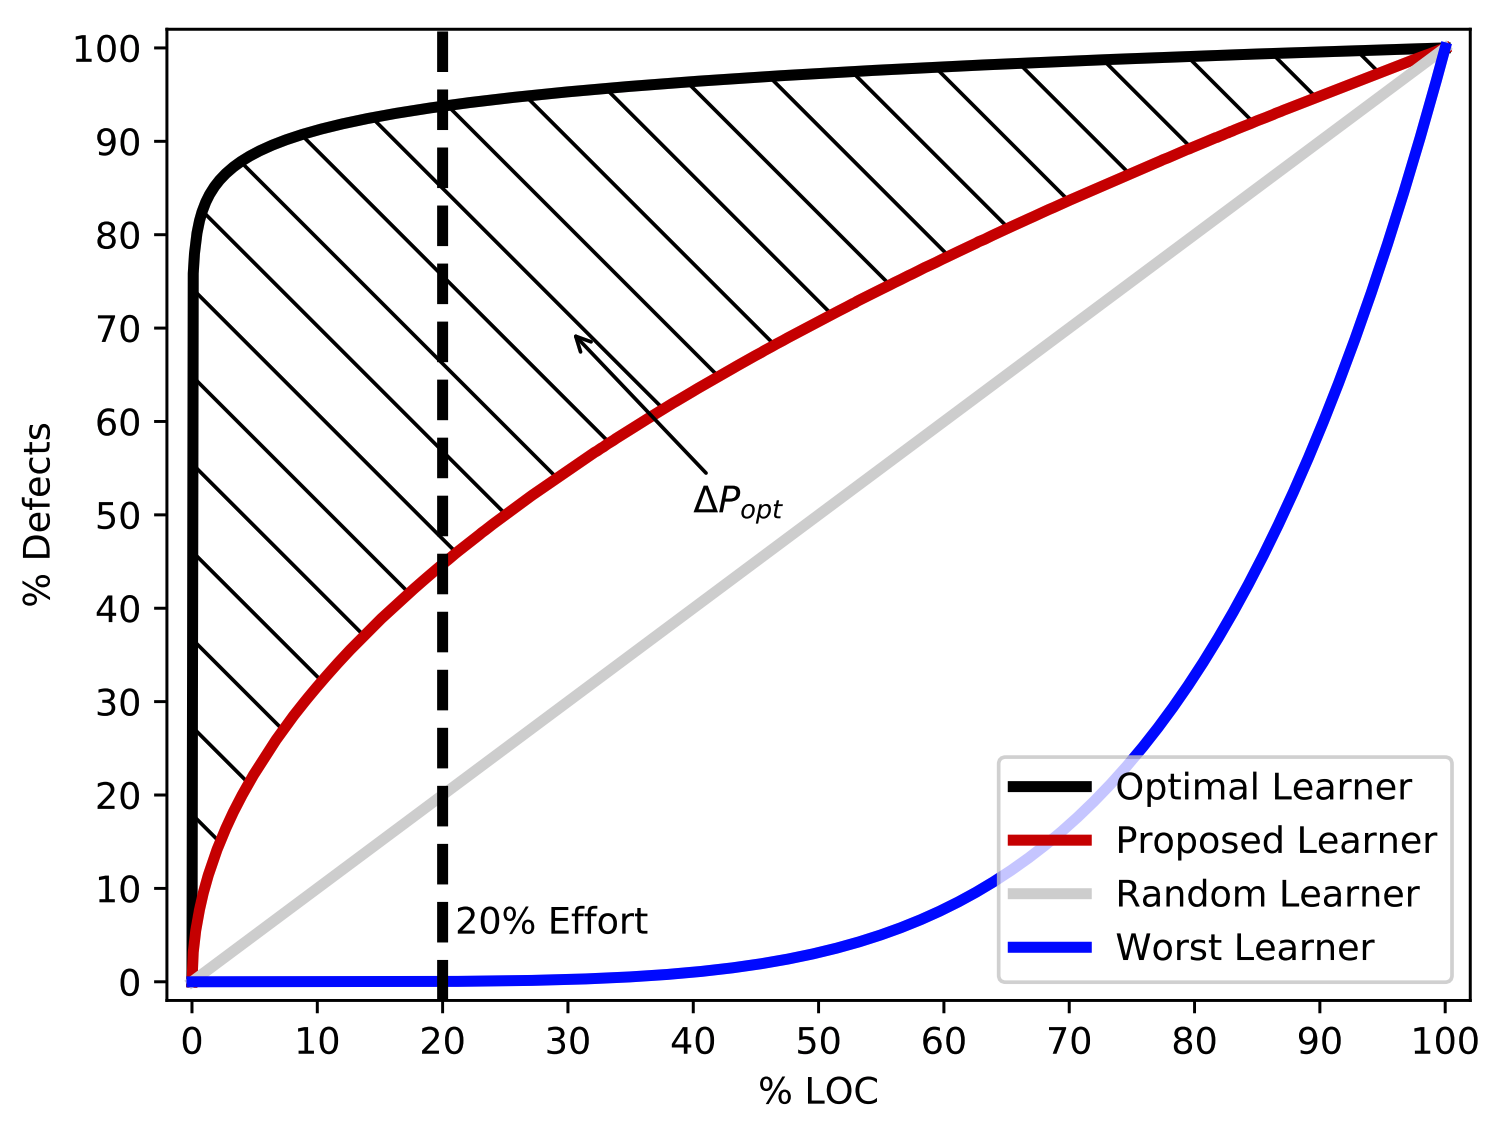
\includegraphics[width=1.65in, height=1.5in]{popt.png}
\vspace{-13pt}
\caption{Effort-based cumulative lift chart}\label{fig:popt}
\vspace{-20pt}
\end{wrapfigure} 

$P_{opt}$ reports the risky software commits have been found by (1) sorting the project components or commits from ``most defect prone'' to ``least likely''; then (2) developers can inspect 20\% the code of the whole project (by lines of code) per commit to find how many risky software commit can be detected by the learner then.  $P_{opt}$ is defined as $1 - \Delta_{opt}$ with $\Delta_{opt}$ as the area between the effort cumulative lift charts of the optimal model and the prediction model (as shown in Figure \ref{fig:popt}). In this chart, the x-axis is the
percentage of required effort to inspect the code and the y-axis is
the percentage of defects found in the selected code. In the optimal
model, all the changes are sorted by the actual defect density, while for the predicted model, all the changes are sorted by the actual predicted value. Both changes are sorted in descending order. The worst model is also built by sorting all the changes according
to the actual defect density in ascending order.
$S(optimal), S(m)$ and $S(worst)$ represent the area of curve
under the optimal model, predicted model, and worst model, respectively. $P_{opt}$ is normalized as  \cite{yang16effort, kamei12_jit, monden13cost}:

\begin{equation}
 \mathit{score_2} = \mathit{P_{opt}(m)} = 1 - \frac{S(optimal) - S(m)}{S(optimal) - S(worst)}
\end{equation}

%\subsection{Statistical Testing}

%We compared our results of tuned miners per release version using statistical significance test and an effect size test by Scott-Knott procedure \cite{mittas2013ranking, ghotra15}. Significance test detects if two populations differ merely by random noises \cite{ghotra15}. Effect sizes checks whether two populations differ by more than just a trivial amount, where $\mathit{A12}$ effect size test was used \cite{arcuri2011practical}. Our stats test are statistically significant with 95\% confidence and not a ``small'' effect ($\mathit{A12} \ge 0.6$).



\section{Results}



\textbf{RQ1: { How close are FASTREAD and Keyword Labeling to Human Labeling?}}
 
Software maintenance is a continuing process and software developers have the domain expertise in understanding the commit logs. Four popular repositories (ABINIT, LAMMPS, LIBMESH, and MDANALYSIS) that satisfies our sanity checks were picked at random and their commit logs were sampled to be labeled for bug-fixing commits by human. With the initial assumption that software maintenance requires the expert's understanding, these human labeled commit logs data from those four repositories serves as the ground truth to compare the effectiveness of automatic keywords tagging versus FASTREAD tagging. Table \ref{tab:rq1} is very clear and we can conclude that FASTREAD won significantly on all three evaluations metrics (precision: 8\%-21\%, recall: 11\%-23\%, and especially in false-alarm 8\%-38\%). Interestingly, between false-alarm and recall relationship, if one metric is optimized, the other usually declined. However, from our initial results on just labeling comparing with manual human ground truths labels, FASTREAD labels to identify software bug-fixing commits are very close to how a developers would label them. 

\begin{RQ}{}
\vspace{-10pt}
FASTREAD as the method for bug-fixing commits augmentation is better than current automatic keyword tagging.
\end{RQ}


\begin{table}[!t]
\caption{FASTREAD (F) vs Keywords (K) for bug-fixing commits identification performance.}
\label{tab:rq1}
\begin{center}
%\begin{threeparttable}
%\vspace{-10pt}
%\resizebox{!}{0.2\linewidth}{
\setlength\tabcolsep{10pt}
\begin{tabular}{ l|c|c|c|c|c|c }
 \multicolumn{1}{c|}{} & \multicolumn{2}{c|}{Precision} & \multicolumn{2}{c|}{Recall} & \multicolumn{2}{c}{False-Alarm}\\
\cline{2-7}
 Dataset & K & F & K & F & K & F \\
\hline
LIBMESH & 79 & 87 & 74 & 97 & 24 & 17 \\
ABINIT & 78 & 86 &  81 & 96 & 29 & 18 \\
MDANALYSIS & 72 & 84  & 84 & 95 & 42 & 23 \\
LAMMPS & 57 & 78  & 81 & 99 & 73 & 35 \\
\end{tabular}
%}
%\end{threeparttable}
\end{center}
\end{table}



\textbf{RQ2: { How are risky software commit prediction based on FASTREAD labeled data perform against state-of-the-art method (Keyword) labeled data?}}
 
 \begin{table}[!t]
\small
\begin{center}
\caption{RQ2 FFT Validation Statistical Results - G-value (top) and $P_{opt}$ (bottom) percentage performance comparison of statistically significant wins across all the releases per project between FFTs versus state-of-the-art methods (SMOTE+SVM, SMOTE+RF, and SMOTE+LR)}
\label{tb:rq4}
\begin{tabular}{c@{~}|r@{~}|r@{~}|r@{~}|r@{~}}
\begin{tabular}[c]{@{}c@{}} \textbf{Dataset} \end{tabular} & \begin{tabular}[c]{@{}c@{}} \textbf{SMOTE+RF}\end{tabular} & \textbf{SMOTE+SVM} & \begin{tabular}[c]{@{}c@{}} \textbf{SMOTE+LR}\end{tabular} & \textbf{FFT} \\ \hline
PCMSOLVER & 0 & 0 & 100 & 0  \\ 
AMBER & 0 & 0 & 33 & 33  \\ 
LAMMPS & 0 & 0 & 0 & 37  \\  
XENON & 0 & 0 & 16 & 50 \\ 
ABINIT & 0 & 0 & 12 & 50  \\  
HOOMD & 0 & 0 & 0 & 60\\ 
RMG-PY & 0 & 0 & 0 & 60\\ 
MDANALYSIS & 0 & 0 & 0 & 71\\ 
LIBMESH & 0 & 0 & 0 & 100\\ 
\end{tabular}
\end{center} 
\vspace{-10pt}
\end{table} 

\begin{table}[!t]
\small
\begin{center}
\begin{tabular}{c@{~}|r@{~}|r@{~}|r@{~}|r@{~}}
\begin{tabular}[c]{@{}c@{}} \textbf{Dataset} \end{tabular} & \begin{tabular}[c]{@{}c@{}} \textbf{SMOTE+RF}\end{tabular} & \textbf{SMOTE+SVM} & \begin{tabular}[c]{@{}c@{}} \textbf{SMOTE+LR}\end{tabular} & \textbf{FFT} \\ \hline
PCMSOLVER & 0 & 0 & 0 & 0  \\ 

LAMMPS & 37 & 0 & 0 & 12  \\  

HOOMD & 0 & 0 & 0 & 20  \\  
MDANALYSIS & 28 & 0 & 0 & 28\\ 
XENON  & 16 & 0 & 0 & 33\\ 
ABINIT & 0 & 0 & 0 & 37 \\ 
LIBMESH & 12 & 0 & 0 & 50\\ 
AMBER & 0 & 33 & 0 & 66  \\ 
RMG-PY & 0 & 0 & 0 & 80\\ 

\end{tabular}
\end{center} 
\vspace{-10pt}
\end{table}

  
From the bug-fixing commits, we can track back to find bug-inducing commits that introducing defects to the software. Each of these commits will be analyzed and recommended metrics are extracted to describe how risky each commit is. Finding the right bug-inducing commits will help to link to the right bug-inducing commits with appropriate values of metrics to build a strong model to predict future risky software commits. Our recommended data mining method is FFT with no preprocessing. Essentially, we wanted to compare $F^3T$ (FASTREAD+FFT) and Keyword+FFT.
 
 
 
 In order to validate our chosen data miner, FFTs, we evaluated the performance of it by building FFTs on FASTREAD labeled data against standard methods (SMOTE+SVM, SMOTE+RF, and SMOTE+LR). Table \ref{tb:rq4} provides the statistical testing results for G-value (top) and $P_{opt}$ (bottom) performances. For G-value, FFT dominated in most of the releases, 7 wins out of 9 projects while performing similarly in 1 case (in AMBER) and losing to SMOTE+LR in 1 case (in PCMSOLVER) when 6 wins have 50\% and above win. For $P_{opt}$, FFT performance also have the most win percentages in most of the releases, 6 wins out of 9 projects while performing similarly to other data mining methods in 2 cases (PCMSOLVER and MDANALYSIS) and losing to SMOTE+RF in 1 case (in LAMMPS).  Figure \ref{fig:rq4} provides the median absolute delta performance insight from each project numerically between FFTs and state-of-the-art data mining methods (SMOTE+RF, SMOTE+SVM, and SMOTE+LR). We can see: (1) RF is widely adopted in defect prediction task but surprisingly doing worst in G-value (when comparing with FFTs for the median delta difference across all releases); (2) The good performance of SMOTE+LR when comparing to SMOTE+RF and SMOTE+SVM in G-value is evidental to why even though LR is deprecated in defect prediction task, it is widely adopted in JIT defect prediction \cite{commitguru}; (3) FFTs model outperformed standard data mining methods is validated as our chosen data miner. 

 \begin{figure}[!t]
\vspace{-10pt}
\caption{RQ2 FFT Validation by Numerical Difference Result - Absolute median delta of G-value (top chart) and $P_{opt}$ (bottom  chart) of comparing the performances between FFTs and state-of-the-art methods (SMOTE+SVM, SMOTE+RF, and SMOTE+LR)}
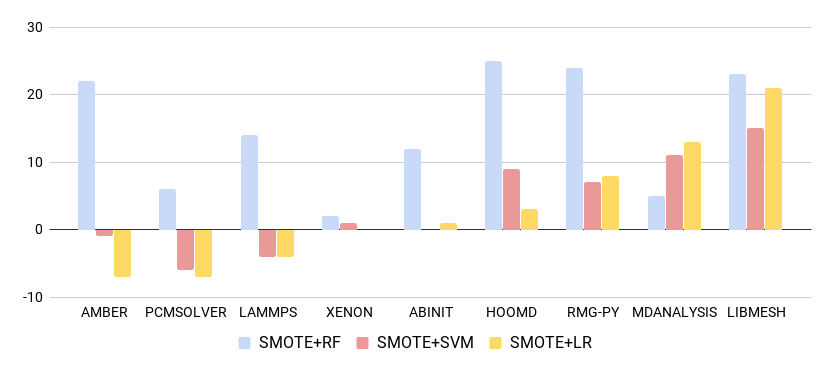
\includegraphics[width=\linewidth, height=1.8in]{rq4_1.png}
\label{fig:rq4}
\vspace{-25pt}
\end{figure}
\begin{figure}[!t]
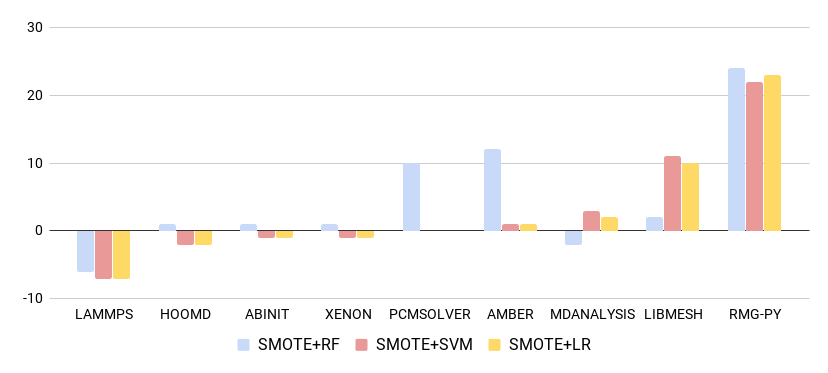
\includegraphics[width=\linewidth, height=1.8in]{rq4_2.png}
\vspace{-25pt}
\end{figure}
 



\begin{figure*}[!t]
\small
\vspace{-10pt}
\caption{RQ2 Numerical Result - Absolute median G-value (top chart) and $P_{opt}$ (bottom chart) performance of comparing the performance using FFTs to build risky software commit prediction on FASTREAD generated data ($F^3T$) versus Keyword generated data (Keyword+FFT) for each release per project.}
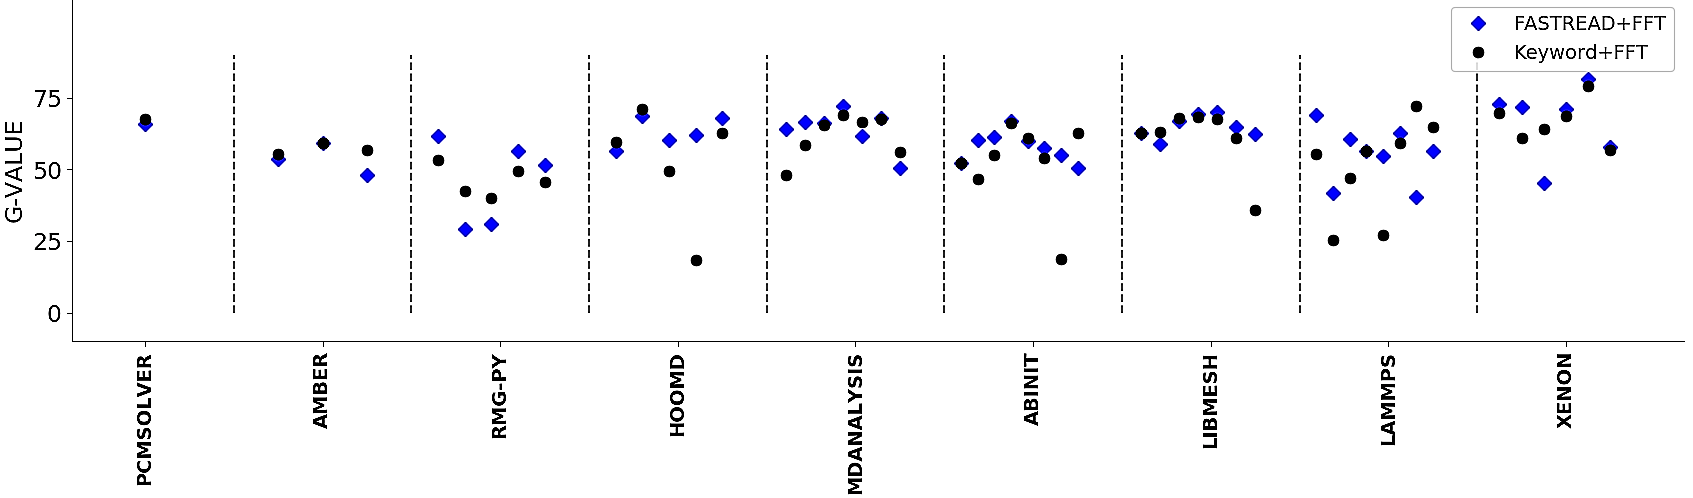
\includegraphics[width=\linewidth, height=1.8in]{rq2_1.png}
\label{fig:rq2}
\vspace{-20pt}
\end{figure*}
\begin{figure*}[!t]
\small
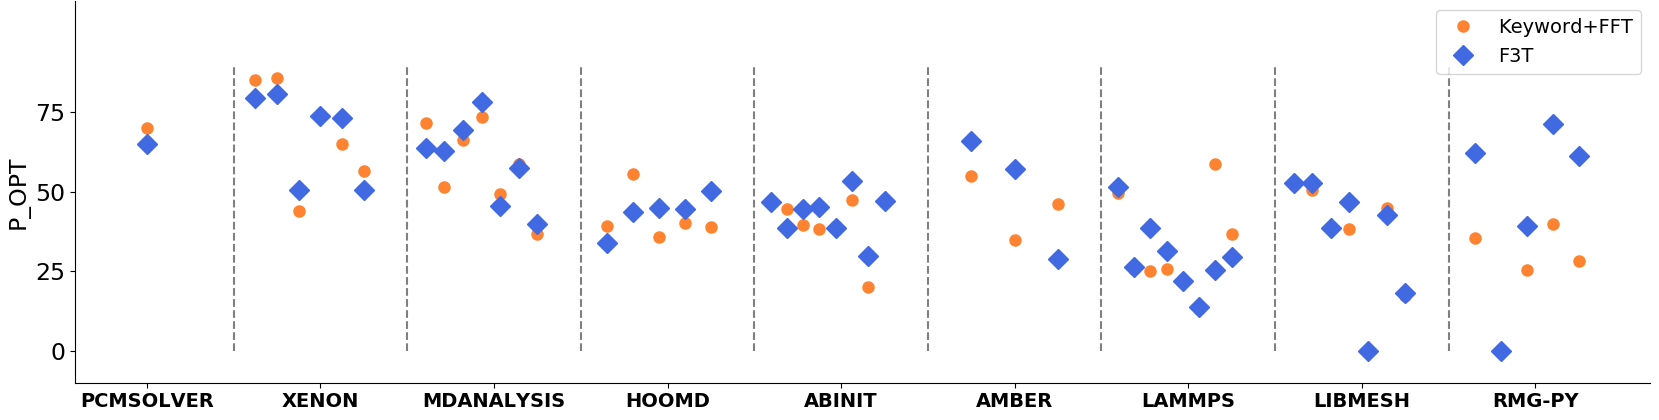
\includegraphics[width=\linewidth, height=1.8in]{rq2_2.png}
\vspace{-20pt}
\end{figure*}


 
 Figure \ref{fig:rq2} provides the median performance insight from each project for each release numerically between $F^3T$ and Keyword+FFT for G-value (top chart) and $P_{opt}$ (bottom chart). The blue diamond represents $F^3T$ while the black circle represents Keyword+FFT A lot of the differences between the two methods are easy to spot (i.e. performance on $P_{opt}$ chart for RMG-PY), but some are not (i.e. performance on G-value chart for AMBER). In order to confirm our hypothesis,
 the percentage of statistically significant winning or ranking higher across all the releases in each project are recorded in Table \ref{tb:rq2}. Specifically, for LAMMPS, there are 9 releases, so the performance metrics are collected 8 times incrementally and FFT model built on FASTREAD generated data won 6/8 for G-value and 4/8 for $P_{opt}$  so $F^3T$ won 75\% time for G-value and 50\% for $P_{opt}$ in LAMMPS. The higher number between the twos is the better combination method. Four initial datasets that got human ground truth labels are expressed in bold entries. We observe that four out four, $F^3T$ statistically overwhelm Keyword+FFT using the "Human labeled" ground truths.  
 

\begin{table}
\small
\begin{center}
\caption{RQ2 Statistical Result - G-value (left) and $P_{opt}$ (right) percentage performance comparison of statistically significant wins across all the releases per project between FASTRERAD+FFT(F+FFT) versus Keyword+FFT(K+FFT)}
\label{tb:rq2}
\resizebox{\linewidth}{!}{
 \begin{minipage}{0.5\linewidth}
\begin{tabular}{c@{~}|r@{~}|r@{~}}
\begin{tabular}[c]{@{}c@{}} \textbf{Dataset} \end{tabular} & \begin{tabular}[c]{@{}c@{}} \textbf{K+FFT}\end{tabular} & \textbf{F+FFT}\\ \hline
PCMSOLVER & 100 & 0  \\ 
AMBER & 67 & 33  \\ 
HOOMD & 40 & 60 \\ 
RMG-PY  & 40 & 60 \\ 
\textbf{ABINIT} & \textbf{25} & \textbf{62} \\ 
\textbf{LIBMESH} & \textbf{28} & \textbf{72}  \\  
\textbf{MDANALYSIS} & \textbf{28} & \textbf{72} \\ 
\textbf{LAMMPS} & \textbf{25} & \textbf{75} \\
XENON & 16 & 83  \\  
\end{tabular}
\end{minipage} \
\begin{minipage}{0.5\linewidth}
\begin{tabular}{c@{~}|r@{~}|r@{~}}
\begin{tabular}[c]{@{}c@{}} \textbf{Dataset} \end{tabular} & \begin{tabular}[c]{@{}c@{}} \textbf{K+FFT}\end{tabular} & \textbf{F+FFT}\\ \hline
AMBER & 67 & 33  \\
HOOMD & 60 & 40 \\ 
XENON & 50 & 50  \\  
\textbf{LAMMPS} & \textbf{37} & \textbf{50} \\
\textbf{ABINIT} & \textbf{37} & \textbf{50} \\ 
\textbf{MDANALYSIS} & \textbf{42} & \textbf{57} \\ 
RMG-PY & 20 & 80 \\ 
\textbf{LIBMESH} & \textbf{14} & \textbf{86}  \\  
PCMSOLVER & 0 & 100  \\ 
\end{tabular}
\end{minipage}}
\end{center} 
\vspace{-10pt}
\end{table}





Manual human labeled ground truths are important for the data mining process but expensive to get and hard to repeat. Original four initial datasets provide plentiful evidence for us to have confidence in FASTREAD generated risky software prediction data. In order to confirm that hypothesis, the experiment is repeated without human ground truth labels by testing only on the next release that was generated from the same labeling method(i.e., a learner that was trained on ABINIT Keyword release 1 will predict on ABINIT Keyword release 2 and a learner that was trained on ABINIT FASTREAD release 1 will be tested on ABINIT FASTREAD release 2). It is similar to previous studies that solely using automating Keyword  \cite{nayrolles18_clever, commitguru}. 


With 7 and 6 wins out of 9 projects for G-value and $P_{opt}$ respectively, FFTs model built on FASTREAD generated data outperformed FFTs model built on Keyword generated data. Hence, 

\begin{RQ}{}
\vspace{-10pt}
FASTREAD labeled data are more fit and higher quality for risky software commit prediction. Automatic Keywords labeling method for defective software commit is deprecated for future defect prediction work.  
\end{RQ}

\begin{table}
\small
\begin{center}
\caption{RQ3 Statistical Result - G-value (left) and $P_{opt}$ (right) percentage performance comparison of statistically significant wins across all the releases per project between $F^3T$ versus Commit.Guru}
\label{tb:rq3}
\resizebox{\linewidth}{!}{
 \begin{minipage}{0.5\linewidth}
\begin{tabular}{c@{~}|r@{~}|r@{~}}
\begin{tabular}[c]{@{}c@{}} \end{tabular} & \begin{tabular}[c]{@{}c@{}} \textbf{Commit}\end{tabular} & \\
\textbf{Dataset}  &  \textbf{Guru} & \textbf{FFFT}\\\hline
XENON & 16 & 66  \\ 
LAMMPS & 0 & 75 \\ 
HOOMD & 20 & 80 \\ 
ABINIT  & 0 & 87 \\ 
AMBER & 0 & 100 \\ 
RMG-PY & 0 & 100 \\ 
LIBMESH & 0 & 100 \\ 
PCMSOLVER & 0 & 100 \\  
MDANALYSIS & 0 & 100  \\ 
\end{tabular} \qquad
\end{minipage}
\begin{minipage}{0.5\linewidth}
\begin{tabular}{c@{~}|r@{~}|r@{~}}
\begin{tabular}[c]{@{}c@{}} \end{tabular} & \begin{tabular}[c]{@{}c@{}} \textbf{Commit}\end{tabular} & \\
\textbf{Dataset}  &  \textbf{Guru} & \textbf{FFFT}\\\hline
PCMSOLVER & 100 & 0  \\ 
AMBER & 67 & 33  \\ 
HOOMD & 40 & 60 \\ 
RMG-PY  & 40 & 60 \\ 
ABINIT & 25 & 62 \\ 
LIBMESH & 28 & 72  \\  
MDANALYSIS & 28 & 72 \\ 
LAMMPS & 25 & 75 \\
XENON & 16 & 83  \\  

\end{tabular}
\end{minipage}}

\end{center} 
\vspace{-20pt}
\end{table}

\begin{figure*}[!t]
\caption{RQ3 Numerical Results - Absolute median G-value (top chart) and $P_{opt}$ (bottom chart) performance of comparing the performance between $F^3T$ and Commit.Guru for each release per project.}
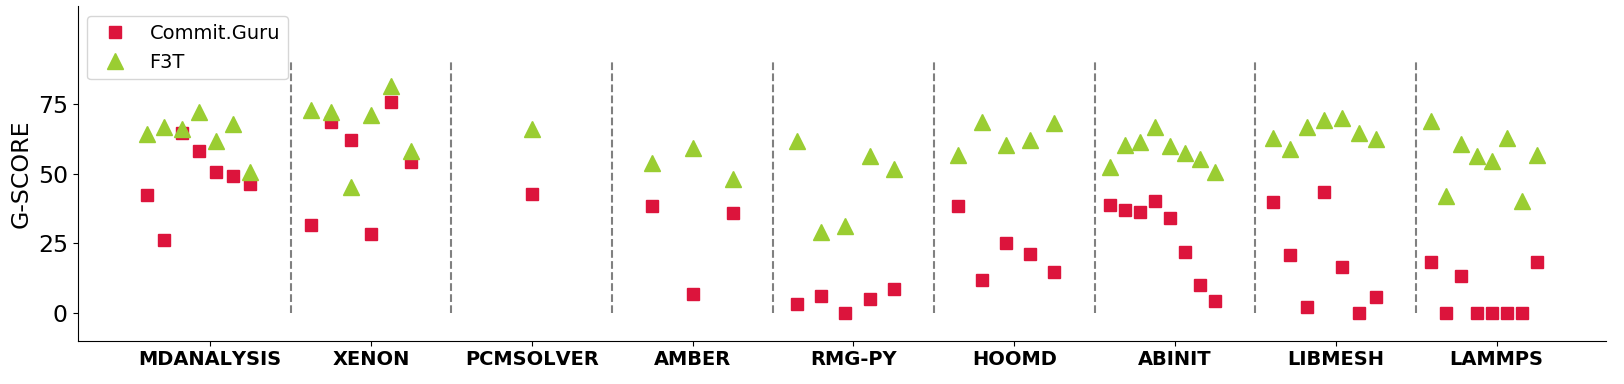
\includegraphics[width=\linewidth, height=1.8in]{rq3_1.png}
\label{fig:rq3}
\vspace{-25pt}
\end{figure*}
\begin{figure*}[!t]
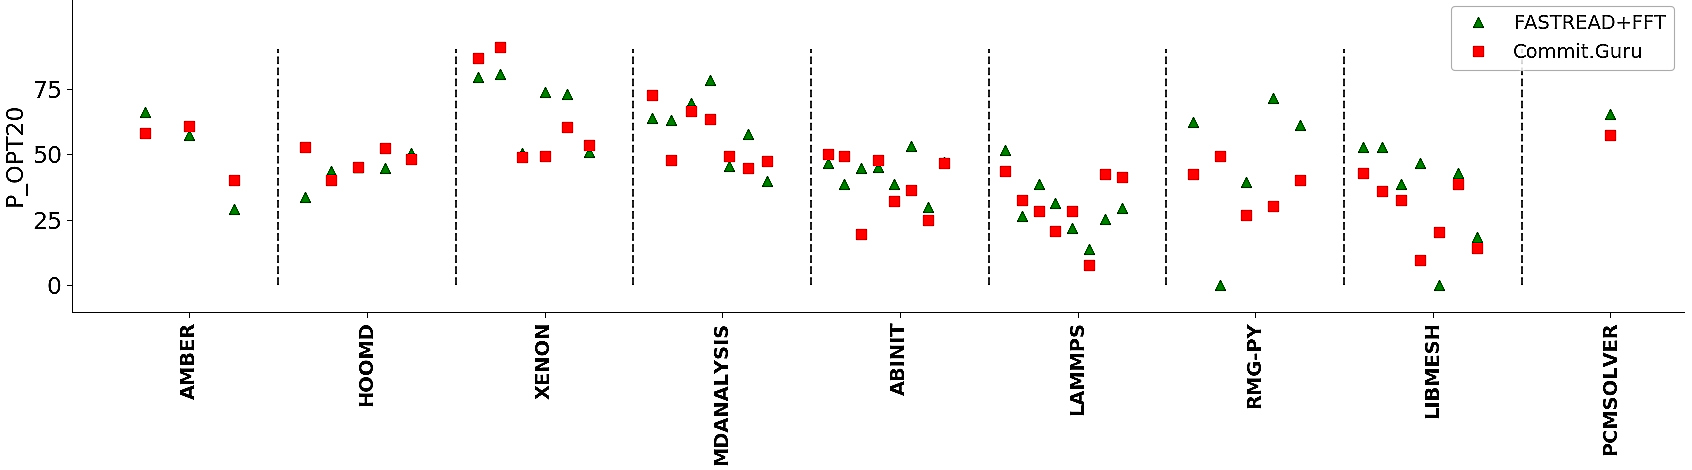
\includegraphics[width=\linewidth, height=1.8in]{rq3_2.png}
\vspace{-20pt}
\end{figure*}

\textbf{RQ3: {How state-of-the-art risky software commit identification and prediction system, Commit.Guru, comparing to our recommended $F^3T$ system in predicting risky software commit?}}
 
Beside dependent ground truth labels, data quality also comes from the proportion of the labels within the dataset. Agrawal et al. \cite{agrawal2018better} has found that the imbalance class problem is apparent within defect prediction research. Although, our study is not defect prediction, it does inherit a lot of defect prediction problem's nature where most of the commits are not bug-inducing commits as shown in Table \ref{tbl:dataset} where the median of defective commit is 23\%. Therefore, risky software commit also exhibit imbalance class problem. Outside of data quality, data miner should be chosen carefully to leverage the nature of the problem and the dataset itself. FASTREAD improves the dependent features quality or the correctness of risky software commit identification, target for prediction task (from RQ1 and RQ2) while FFTs model has proven to be a strong data miner for software analytics task. Our recommended $F^3T$ method is chosen for this paper to compare against state-of-the-art risky software prediction method, Commit.Guru's Keyword+LR. 

From the Figure \ref{fig:rq3}, the green triangles and red squares represent $F^3T$'s performance and Commit.Guru's performance for G-value (top chart) and $P_{opt}$ (bottom chart). $F^3T$ clearly outperformed Keyword+LR on all 9 projects for G-value where $F^3T$ won 100\% of the time in 5 projects for all the releases within that same project (recorded Table \ref{tb:rq3}). For $P_{opt}$ $F^3T$ won 7 out of 9 projects for $P_{opt}$ with statistically significant different in the right of Table \ref{tb:rq3}. With the majority won on both measures, we can conclude: 


\begin{RQ}{}
\vspace{-10pt}
$F^3T$ outperformed state-of-the-art risky software commit identification and prediction system, Commit.Guru. $F^3T$ is recommended as a new baseline for future research work.
\end{RQ}




% \textbf{RQ4: { How FFT model comparing to state-of-the-art data mining methods in predicting risky software commit?}}
 
% Modern state-of-the-art methods does include more than just Logistic Regression such as Random Forest and Support Vector Machine for more complex problems in the combination with Synthetic Minority Oversampling Technique (SMOTE) to handle class imbalance problem. It is essential to validate our data miner of choice (i.e. FFTs), by comparing against state-of-the-art data mining methods in SE research. 

% \begin{figure}[!t]
% \vspace{-10pt}
% \caption{RQ4 Numerical Difference Result - Absolute median delta of G-value (top chart) and $P_{opt}$ (bottom  chart) of comparing the performances between FFTs and state-of-the-art methods (SMOTE+SVM, SMOTE+RF, and SMOTE+LR)}
% 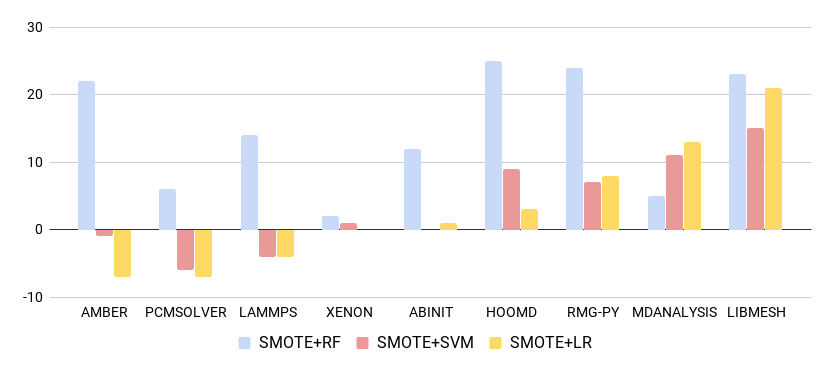
\includegraphics[width=\linewidth, height=1.8in]{rq4_1.png}
% \label{fig:rq4}
% \vspace{-25pt}
% \end{figure}
% \begin{figure}[!t]
% 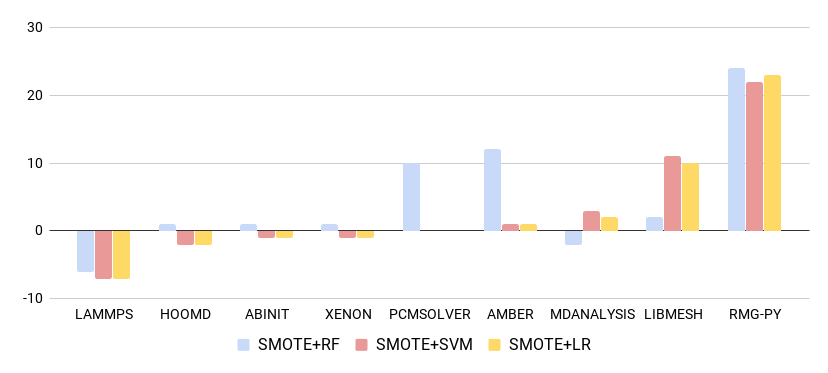
\includegraphics[width=\linewidth, height=1.8in]{rq4_2.png}
% \vspace{-25pt}
% \end{figure}

% The experiment and evaluation are similar to RQ2 and RQ3 but only training and testing on FASTREAD generated data. Table \ref{tb:rq4} provides the statistical testing results for G-value (top) and $P_{opt}$ (bottom) performances of comparing FFTs with SMOTE+RF, SMOTE+SVM, and SMOTE+LR. For G-value, FFT dominated in most of the releases, 7 wins out of 9 projects while performing similarly in 1 case (in AMBER) and losing to SMOTE+LR in 1 case (in PCMSOLVER) when 6 wins have 50\% and above win. For $P_{opt}$, FFT performance also have the most win percentages in most of the releases, 6 wins out of 9 projects while performing similarly to other data mining methods in 2 cases (PCMSOLVER and MDANALYSIS) and losing to SMOTE+RF in 1 case (in LAMMPS).  Figure \ref{fig:rq4} provides the median absolute delta performance insight from each project numerically between FFTs and state-of-the-art data mining methods (SMOTE+RF, SMOTE+SVM, and SMOTE+LR). We can see: (1) RF is widely adopted in defect prediction task but surprisingly doing worst in G-value (when comparing with FFTs for the median delta difference across all releases); (2) The good performance of SMOTE+LR when comparing to SMOTE+RF and SMOTE+SVM in G-value is evidental to why even though LR is deprecated in defect prediction task, it is  widely adopted in JIT defect prediction \cite{commitguru}. Finally, 


% \begin{RQ}{}
% \vspace{-10pt}
% FFT model outperformed state-of-the-art risky software commit prediction and is recommended as a new baseline for future work in risky software commit prediction.
% \end{RQ}







\section{Threats to Validity }

\subsection{Sampling Bias}

Our data mining work do share the sampling bias nature as other data mining work. What hold importance in one situation may not hold in another. 9 open-source projects were considered with more than $36,000+$ post-preprocessed change commits but not all of them covering the full project development (some are subsets). There exists different ways to decide how a release is a major one where we rely on the naming convention and size of the release to group different releases together. In order to reduce sampling bias nature:

\bi
\item An executable reproduction package and documentation will be available for all experimentation. 
\item When new data becomes available, we can test our methods on the new data. 
\ei



\subsection{Learner Bias}

For building risky software commit prediction, Logistic Regression, Random Forest, and Support Vector Machine with the combination of SMOTE are elected. They represented different categories in defect prediction tasks but also are state-of-the-art method to be evaluated for risky software commit prediction. 

\subsection{Evaluation Bias}

This paper employed G-score as defined in Equation 3 as the harmonic mean between recall and false-alarm of risky software commit prediction power. Other evaluation measure that have been proven to quantify the effectiveness of prediction \cite{} and can be implemented conveniently to extend the work through the reproduction package of this paper.   

\subsection{Order Bias}

For the performance evaluation part, the order that the data trained and predicted affects the results.
For this risky software commit prediction datasets, an ordering is deliberately chosen to mimic how a software is developed which leads to that our bias is required and needed. 

\section{Conclusion}

The market for software tools and services are drastically growing. After creation, comes software maintenance. Software maintenance is an endless and continuing process in which software developers have the domain expertise for identifying the defect-prone code/subsystems/commits. Beside source code analysis, source code logs/comments/commits are essential to reason the defect rate of a system. However, current state-of-the-art quality and risk prediction of software commits augmenting the data by simply checking for the existing of defect-related keywords within the commit message which has been found to have low accuracy even with the help of topic modeling model. We introduced $F^3T$ system for JIT software quality assurance with (1) FASTREAD for bug-inducing commits identification and (2) FFT as the data miner for risky software commit prediction where:

\bi
\item With human-labeled as ground-truths, FASTREAD maximizes recall and minimizes false-alarm for bug-fixing commits identification more than automatic Keyword tagging method.
\item FASTREAD provides higher quality data for better performance of risky software commit prediction model (i.e. FFT) than Keyword when evaluating with G-value and $P_{opt}$.  
\item $F^3T$ system remarkably outperform state-of-the-art Commit.Guru for risky software commits prediction. 
\ei

From our study empirical results, we recommend:
\begin{enumerate}
    \item Commit messages/logs have complex nature but are important to software maintenance and should not be done automatically through keywords tagging. A human-in-the-loop AI method utilizing active learner such as FASTREAD is recommended for defect-prone commits reviewing.   
    \item FFT should be considered as a baseline for future work in risky software commits prediction. 
\end{enumerate} 



\balance
\bibliographystyle{ACM-Reference-Format}

% \bibliographystyle{plain}
% \bibliography{reference}

\bibliography{sample.bib}



\end{document}